\documentclass[14pt]{extbook}
\usepackage{multicol, enumerate, enumitem, hyperref, color, soul, setspace, parskip, fancyhdr} %General Packages
\usepackage{amssymb, amsthm, amsmath, latexsym, units, mathtools} %Math Packages
\everymath{\displaystyle} %All math in Display Style
% Packages with additional options
\usepackage[headsep=0.5cm,headheight=12pt, left=1 in,right= 1 in,top= 1 in,bottom= 1 in]{geometry}
\usepackage[usenames,dvipsnames]{xcolor}
\usepackage{dashrule}  % Package to use the command below to create lines between items
\newcommand{\litem}[1]{\item#1\hspace*{-1cm}\rule{\textwidth}{0.4pt}}
\pagestyle{fancy}
\lhead{Progress Quiz 3}
\chead{}
\rhead{Version C}
\lfoot{3012-8528}
\cfoot{}
\rfoot{Summer C 2021}
\begin{document}

\begin{enumerate}
\litem{
Find the equation of the line described below. Write the linear equation in the form $ y=mx+b $ and choose the intervals that contain $m$ and $b$.\[ \text{Perpendicular to } 8 x + 7 y = 15 \text{ and passing through the point } (3, -8). \]\begin{enumerate}[label=\Alph*.]
\item \( m \in [-0.92, -0.76] \hspace*{3mm} b \in [-6.66, -5.11] \)
\item \( m \in [0.74, 1.04] \hspace*{3mm} b \in [9.9, 11.01] \)
\item \( m \in [0.74, 1.04] \hspace*{3mm} b \in [-10.91, -9.65] \)
\item \( m \in [1.02, 1.16] \hspace*{3mm} b \in [-10.91, -9.65] \)
\item \( m \in [0.74, 1.04] \hspace*{3mm} b \in [-11.81, -10.68] \)

\end{enumerate} }
\litem{
Solve the equation below. Then, choose the interval that contains the solution.\[ -13(-8x -16) = -10(2x + 19) \]\begin{enumerate}[label=\Alph*.]
\item \( x \in [-3.24, -3.16] \)
\item \( x \in [0.01, 0.16] \)
\item \( x \in [-0.21, -0.14] \)
\item \( x \in [-0.26, -0.2] \)
\item \( \text{There are no real solutions.} \)

\end{enumerate} }
\litem{
Write the equation of the line in the graph below in Standard Form $Ax+By=C$. Then, choose the intervals that contain $A, B, \text{ and } C$.
\begin{center}
    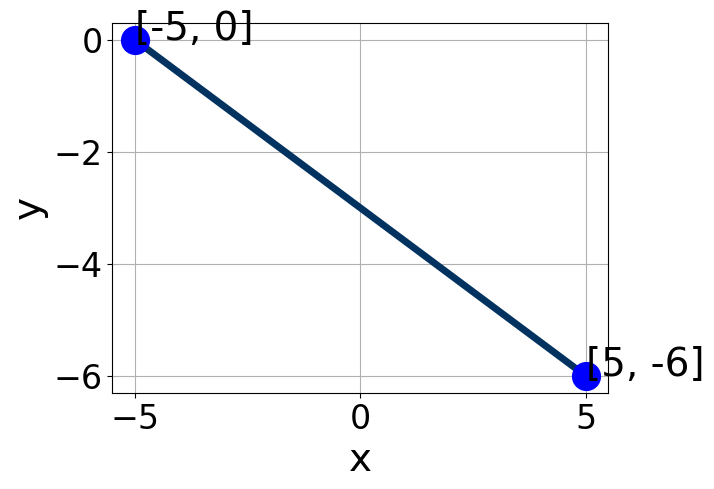
\includegraphics[width=0.5\textwidth]{../Figures/linearGraphToStandardCopyC.png}
\end{center}
\begin{enumerate}[label=\Alph*.]
\item \( A \in [0, 2.7], \hspace{3mm} B \in [-4, 0.2], \text{ and } \hspace{3mm} C \in [1, 8] \)
\item \( A \in [-3.6, -2.9], \hspace{3mm} B \in [-5.5, -3.2], \text{ and } \hspace{3mm} C \in [13, 18] \)
\item \( A \in [0.8, 3.7], \hspace{3mm} B \in [-5.5, -3.2], \text{ and } \hspace{3mm} C \in [13, 18] \)
\item \( A \in [0, 2.7], \hspace{3mm} B \in [-0.2, 2], \text{ and } \hspace{3mm} C \in [-12, 1] \)
\item \( A \in [0.8, 3.7], \hspace{3mm} B \in [3.3, 6], \text{ and } \hspace{3mm} C \in [-15, -13] \)

\end{enumerate} }
\litem{
Find the equation of the line described below. Write the linear equation in the form $ y=mx+b $ and choose the intervals that contain $m$ and $b$.\[ \text{Parallel to } 5 x - 9 y = 12 \text{ and passing through the point } (-7, -8). \]\begin{enumerate}[label=\Alph*.]
\item \( m \in [-0.28, 0.66] \hspace*{3mm} b \in [-6.11, -3.11] \)
\item \( m \in [-0.99, 0.16] \hspace*{3mm} b \in [-18.89, -10.89] \)
\item \( m \in [-0.28, 0.66] \hspace*{3mm} b \in [-3, 2] \)
\item \( m \in [1.69, 2.14] \hspace*{3mm} b \in [-6.11, -3.11] \)
\item \( m \in [-0.28, 0.66] \hspace*{3mm} b \in [2.11, 7.11] \)

\end{enumerate} }
\litem{
Write the equation of the line in the graph below in Standard Form $Ax+By=C$. Then, choose the intervals that contain $A, B, \text{ and } C$.
\begin{center}
    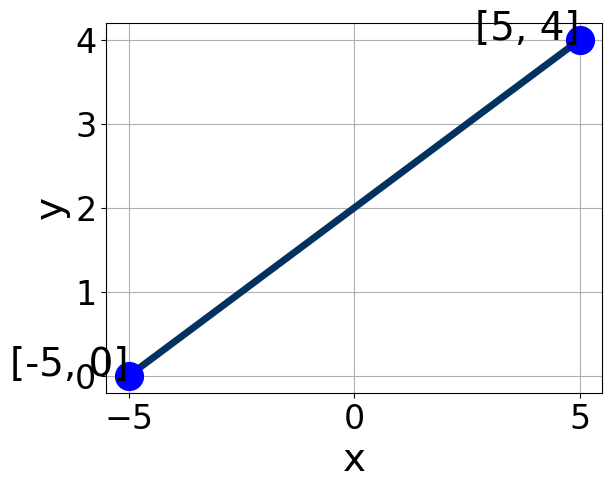
\includegraphics[width=0.5\textwidth]{../Figures/linearGraphToStandardC.png}
\end{center}
\begin{enumerate}[label=\Alph*.]
\item \( A \in [-0.63, 1.12], \hspace{3mm} B \in [-0.2, 2.36], \text{ and } \hspace{3mm} C \in [1, 6] \)
\item \( A \in [1.99, 4.03], \hspace{3mm} B \in [-5.17, -4.42], \text{ and } \hspace{3mm} C \in [-12, -6] \)
\item \( A \in [1.99, 4.03], \hspace{3mm} B \in [3.95, 6], \text{ and } \hspace{3mm} C \in [5, 17] \)
\item \( A \in [-2.3, -1.15], \hspace{3mm} B \in [3.95, 6], \text{ and } \hspace{3mm} C \in [5, 17] \)
\item \( A \in [-0.63, 1.12], \hspace{3mm} B \in [-1.75, 0.36], \text{ and } \hspace{3mm} C \in [-4, 1] \)

\end{enumerate} }
\litem{
Solve the linear equation below. Then, choose the interval that contains the solution.\[ \frac{4x -3}{3} - \frac{6x + 7}{5} = \frac{3x -9}{2} \]\begin{enumerate}[label=\Alph*.]
\item \( x \in [-0.13, 0.75] \)
\item \( x \in [-1.8, -0.58] \)
\item \( x \in [2.51, 3.64] \)
\item \( x \in [0.71, 1.83] \)
\item \( \text{There are no real solutions.} \)

\end{enumerate} }
\litem{
First, find the equation of the line containing the two points below. Then, write the equation in the form $ y=mx+b $ and choose the intervals that contain $m$ and $b$.\[ (-4, 9) \text{ and } (4, 3) \]\begin{enumerate}[label=\Alph*.]
\item \( m \in [-2.1, -0.3] \hspace*{3mm} b \in [4.1, 7.43] \)
\item \( m \in [-2.1, -0.3] \hspace*{3mm} b \in [-1.77, -0.34] \)
\item \( m \in [0.2, 2.7] \hspace*{3mm} b \in [-0.68, 0.44] \)
\item \( m \in [-2.1, -0.3] \hspace*{3mm} b \in [-7.52, -3.78] \)
\item \( m \in [-2.1, -0.3] \hspace*{3mm} b \in [12.59, 13.66] \)

\end{enumerate} }
\litem{
Solve the linear equation below. Then, choose the interval that contains the solution.\[ \frac{-7x + 7}{2} - \frac{-4x + 9}{3} = \frac{-5x -7}{7} \]\begin{enumerate}[label=\Alph*.]
\item \( x \in [-2.2, 0.9] \)
\item \( x \in [1.4, 3.9] \)
\item \( x \in [0.7, 2.3] \)
\item \( x \in [5.1, 6] \)
\item \( \text{There are no real solutions.} \)

\end{enumerate} }
\litem{
Solve the equation below. Then, choose the interval that contains the solution.\[ -6(-18x + 3) = -10(-15x + 19) \]\begin{enumerate}[label=\Alph*.]
\item \( x \in [4.67, 5.4] \)
\item \( x \in [0.28, 1.26] \)
\item \( x \in [2.94, 4.46] \)
\item \( x \in [-6.68, -4.65] \)
\item \( \text{There are no real solutions.} \)

\end{enumerate} }
\litem{
First, find the equation of the line containing the two points below. Then, write the equation in the form $ y=mx+b $ and choose the intervals that contain $m$ and $b$.\[ (9, -10) \text{ and } (3, 11) \]\begin{enumerate}[label=\Alph*.]
\item \( m \in [-4.5, -1.5] \hspace*{3mm} b \in [-21.5, -20.5] \)
\item \( m \in [-4.5, -1.5] \hspace*{3mm} b \in [-20, -18] \)
\item \( m \in [-4.5, -1.5] \hspace*{3mm} b \in [16.5, 24.5] \)
\item \( m \in [-4.5, -1.5] \hspace*{3mm} b \in [5, 16] \)
\item \( m \in [-2.5, 12.5] \hspace*{3mm} b \in [0.5, 2.5] \)

\end{enumerate} }
\end{enumerate}

\end{document}